\section{Durchf\"uhrung}
\label{sec:Durchfuehrung}

\begin{figure}
	\centering
	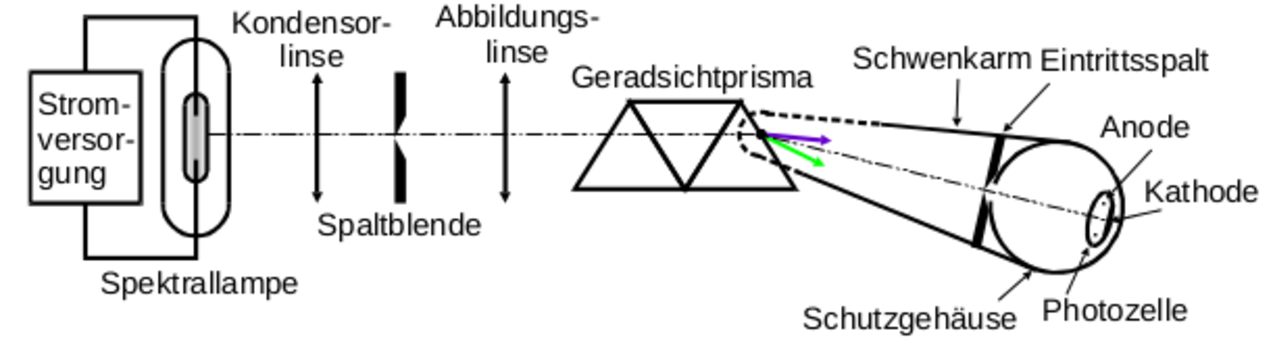
\includegraphics[width=0.9\textwidth]{Bilder/Aufbau.pdf}
	\caption{Anordnung der optischen Elemente zur Untersuchung des Photoeffekts. \cite{skript}}
	\label{fig:Aufbau}
\end{figure}
In Abbildung \ref{fig:Aufbau} ist der gesamte Versuchsaufbau dargestellt. 
Es werden optische Elemente genutzt, um die Intensität des auf die Photozelle fallenden Lichtes zu maximieren. 
Durch geringe Variation der verschiedenen Abstände kann die Anordnung so verändert werden, dass dies gut gelingt. 
Verwendet wird eine Hg-Spektrallampe.
Ihr Licht wird durch eine Kondensorlinse gebündelt und auf einen schmalen Spalt geworfen. 
Bestenfalls befindet sich dieser im Brennpunkt des durch die Linse gebeugten Lichts.
Anschließend passiert das Licht Abbildungslinse und Geradsichprisma. 
Das Prisma bricht das Licht in einzelne Spektrallinien auf. 
Auf einem Schwenkarm sitzt die Photozelle, deren Aufbau in Abbildung \ref{fig:Photozelle} zu sehen ist. 

\begin{figure}[H]
	\centering
	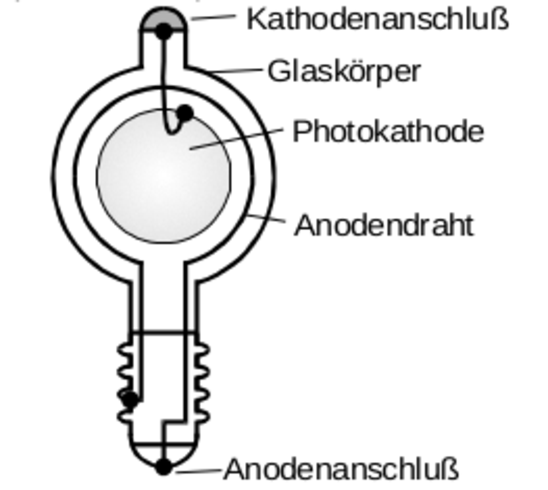
\includegraphics[width=0.4\textwidth]{Bilder/Schema_Photozelle.pdf}
	\caption{Anordnung der optischen Elemente zur Untersuchung des Photoeffekts. \cite{skript}}
	\label{fig:Photozelle}
\end{figure}
Innerhalb der Photozelle befindet sich in einem evakuierten Glasgefäß die im Versuch mit Licht bestrahlte Photokothode. 
In wenigen Millimetern Abstand parallel zur Kathode verweilt die Anode, realisiert durch einen Drahtring, welcher die Kathode umgibt. 
Der Photostrom $I$ wird über ein empfindliches Picoamperemeter gemessen; die Sapnnung $U_\mathup{G}$ kann über ein Digitalvoltmeter variiert werden. 
Das Schaltbild entspricht Abbildung \ref{fig:schaltbild}. 

\begin{figure}[h]
	\centering
	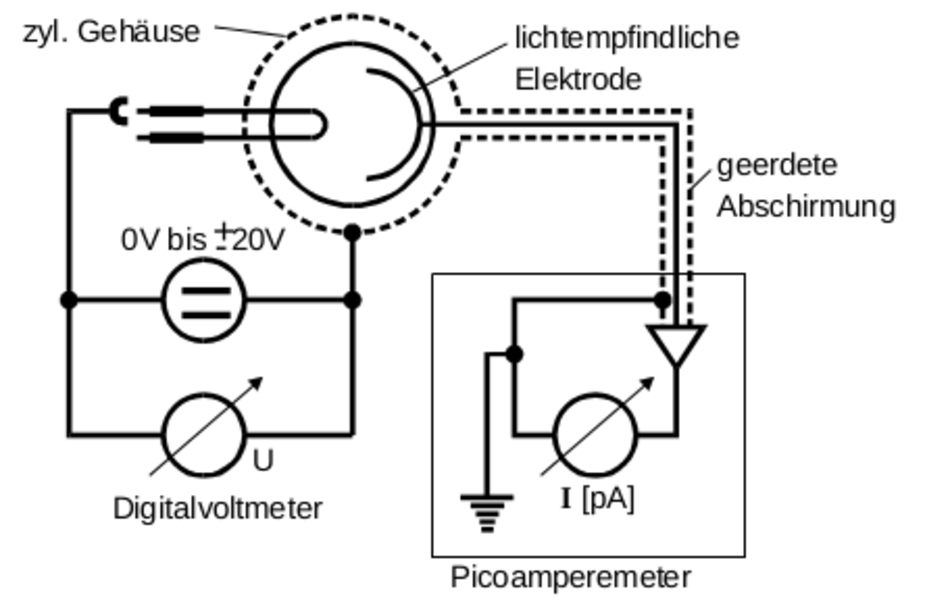
\includegraphics[width=0.5\textwidth]{Bilder/Schaltbild.pdf}
	\caption{Anordnung der optischen Elemente zur Untersuchung des Photoeffekts. \cite{skript}}
	\label{fig:schaltbild}
\end{figure}
Es werden für fünf verschiedene Spektrallinien mindestens 15 Wertepaare $\left(U_\mathup{G},\,I\right)$ aufgenommen, indem die Gegenspannung in regelmäßigen Abständen vergrößert und $I$ abgelesen wird.
Vor dem  eigentlichem Messbeginn wird bei ausgeschalteter Gegenspannung die Photozelle so ausgerichtet, dass die Intensität des Lichts der gewählten Spektrallinie möglichst groß ist. 
Danach wird $U_\mathup{G}$ grob so bestimmt, dass $I=\SI{0}{\volt}$ gilt. 
Alsdann kann mit der eigentlichen Messung begonnen werden.
In einer weiteren Messung wird für die gelbe Spektrallinie der Photostrom über einen Bereich von $\SI{-19}{\volt}\leqslant U_\mathup{G}\leqslant \SI{19}{\volt}$ ausgemessen.
\newpage